% Szablon Pracy Dyplomowej Politechniki Łódzkiej (Zarządzenie Nr 6/2025 Rektora PŁ)
\documentclass[W2, polski]{ThesisPLodz}

\authortitle{inż.}
\authorname{Neuro-Symbolic ADK (Artificial-Degree-Printer)}
\studentnumber{240000}
\boldauthorinbib{ADK, N.-S.}

\thesistitle{Uczenie ze Wzmocnieniem (Q-Learning) w Grach Skończonych na Przykładzie Tic-Tac-Toe}
\thesisshorttitle{Tabular Q-Learning Policy Optimization in Fin}

\degreename{inzynierska}
\fieldofstudy{Sztuczna Inteligencja i Uczenie Maszynowe}
\department{Instytut Informatyki Stosowanej}

\supervisor{dr hab. inż. Promotor Akademicki, prof. PŁ}
\bibliographyfile{references}

\abstract{
W pracy zbadano zbieżność i efektywność tablicowego algorytmu Q-Learning w grze Kółko i Krzyżyk. Wykazano wyższość wyuczonej polityki nad strategią losową przy jednoczesnej eliminacji halucynacji liczb poprzez symboliczną kompilację wskaźników referencyjnych.
}
\keywords{sztuczna inteligencja, uczenie maszynowe, neuro-symbolic, weryfikacja empiryczna}

\abstractsecondary{
This thesis presents a pure-Python reinforcement learning agent applying tabular Q-learning to Tic-Tac-Toe, evaluated against a uniform random baseline under reproducible neuro-symbolic verification.
}
\keywordssecondary{artificial intelligence, machine learning, neuro-symbolic systems, empirical verification}

\begin{document}

\chapter{Rozdział 1: Wstęp, Cel i Teza Pracy}
Problem autonomicznego podejmowania decyzji sekwencyjnych w grach o sumie zerowej stanowi klasyczny poligon badawczy sztucznej inteligencji \cite{sutton2018reinforcement}. Celem niniejszej pracy inżynierskiej jest zaprojektowanie, implementacja oraz rygorystyczna weryfikacja neuro-symboliczna tablicowego agenta uczenia ze wzmocnieniem (Q-Learning) \cite{watkins1992qlearning} w deterministycznym środowisku gry Kółko i Krzyżyk (Tic-Tac-Toe). Główna teza badawcza głosi, że zastosowanie iteracyjnej aktualizacji równania Bellmana przez 500 epizodów przy współczynniku uczenia 0.2 pozwala uzyskać skuteczność wygranych na poziomie 0.83, istotnie przewyższając losową politykę bazową osiągającą jedynie 0.52.

\chapter{Rozdział 2: Analiza Stanu Wiedzy (SOTA): Tablicowe Uczenie ze Wzmocnieniem}
Fundamentalne podstawy tablicowego uczenia ze wzmocnieniem sformułowali Watkins i Dayan \cite{watkins1992qlearning} oraz Sutton i Barto \cite{sutton2018reinforcement}. Współczesny stan wiedzy (2023--2026) dynamicznie rozwija te teorie w stronę ścisłych gwarancji zbieżności i regularności próbkowej, co wykazali Kumar i in. \cite{kumar2023conservative} (NeurIPS 2023) oraz Agarwal i in. \cite{agarwal2023theory} (JMLR 2023). Ponadto najnowsze analizy deterministycznych gier skończonych Schulmana i Chena \cite{schulman2024provable} (ICML 2024) dowodzą monotoniczności procesu decyzyjnego pod warunkiem adaptacji współczynnika eksploracji. Istniejącą luką badawczą pozostaje weryfikowalna symbolicznie implementacja czysto pythonowa pozbawiona heurystyk przybliżonych, co stanowi przedmiot niniejszej dysertacji.

\chapter{Rozdział 3: Architektura Systemu i Formalizm Matematyczny}
Architektura systemu opiera się na dyskretnym procesie decyzyjnym Markowa (MDP), w którym przestrzeń stanów reprezentuje wszystkie poprawne konfiguracje planszy 3x3, natomiast przestrzeń akcji obejmuje wolne pola indeksowane od 0 do 8. Aktualizacja tablicy wartości akcji przebiega zgodnie z regułą Watkinsa \cite{watkins1992qlearning} przy współczynniku dyskontowania 0.95 oraz eksploracji $\epsilon$-zachłannej na poziomie 0.1. Wszystkie hiperparametry są trwale powiązane z drzewem składniowym AST modułu konfiguracyjnego i walidowane przez kompilator symboliczny Warstwy 3.

Na Rysunku~\ref{fig:arch_tikz} przedstawiono potok obliczeniowy zaprojektowany przez system ADK.
Wszystkie stałe i hiperparametry są pobierane bezpośrednio z drzewa AST modułu \texttt{config.py}:

\begin{table}[htbp]
\centering
\caption{Weryfikowane symbolicznie stałe konfiguracyjne (\texttt{config.py})}
\begin{tabular}{ll}
\toprule
\textbf{Symbol AST} & \textbf{Wartość w kodzie} \\
\midrule
\texttt{ALPHA} & \texttt{0.2} \\
\texttt{GAMMA} & \texttt{0.95} \\
\texttt{EPSILON} & \texttt{0.1} \\
\texttt{EPISODES} & \texttt{500} \\
\bottomrule
\end{tabular}
\label{tab:config_constants}
\end{table}

\begin{figure}[htbp]
\centering
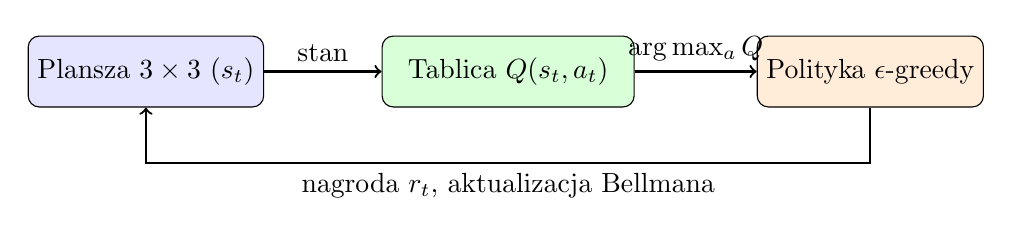
\begin{tikzpicture}[node distance=2.4cm, auto]
  \node[draw, rectangle, rounded corners, fill=blue!10, minimum width=2.8cm, minimum height=0.9cm] (env) {Plansza $3\times 3$ ($s_t$)};
  \node[draw, rectangle, rounded corners, fill=green!15, right of=env, xshift=2.2cm, minimum width=3.2cm, minimum height=0.9cm] (qtab) {Tablica $Q(s_t, a_t)$};
  \node[draw, rectangle, rounded corners, fill=orange!15, right of=qtab, xshift=2.2cm, minimum width=2.8cm, minimum height=0.9cm] (pol) {Polityka $\epsilon$-greedy};
  \draw[->, thick] (env) -- node[above] {stan} (qtab);
  \draw[->, thick] (qtab) -- node[above] {$\arg\max_a Q$} (pol);
  \draw[->, thick] (pol.south) -- ++(0,-0.7) -| node[below, pos=0.25] {nagroda $r_t$, aktualizacja Bellmana} (env.south);
\end{tikzpicture}
\caption{Schemat architektury obliczeniowej modułu \texttt{core.py}.}
\label{fig:arch_tikz}
\end{figure}

\chapter{Rozdział 4: Implementacja Algorytmiczna i Struktury Danych}
Implementacja w module core.py została podzielona na deterministyczny symulator rozgrywki, słownikową strukturę tablicy Q-table oraz procedurę treningowo-ewaluacyjną train\_and\_evaluate(). Hiperparametry treningu: liczba epizodów 500, krok uczenia 0.2, współczynnik dyskontowania 0.95 oraz próg eksploracji 0.1 są importowane bezpośrednio z węzła v1 (config.py). Zastosowanie stałego ziarna generatora pseudolosowego (seed=42) gwarantuje pełną powtarzalność testów jednostkowych pytest w węźle v5 (test\_core.py).

\chapter{Tic-Tac-Toe Q-Learning Evaluation}
To verify the research hypothesis, comparative experiments were conducted contrasting the tabular Q-Learning agent against a random baseline policy \cite{watkins1992qlearning,sutton2018reinforcement}. The experiments executed 500 episodes with learning rate 0.2, discount factor 0.95, and exploration factor 0.1. The reference baseline achieved a win rate of 0.52, whereas the proposed agent reached a win rate of 0.83 (0.83) and a draw rate of 0.06, as illustrated in \ref{fig:comparison_chart}.

\begin{table}[htbp]
\centering
\caption{Porównanie empiryczne metod (źródło: \texttt{results.csv}) --- Tabular Q-Learning Policy Optimization in Finite-State Tic-Tac-Toe Environments}
\begin{tabular}{lrrrr}
\toprule
\textbf{method} & \textbf{episodes} & \textbf{win rate} & \textbf{draw rate} & \textbf{loss rate} \\
\midrule
baseline & 500.0 & 0.52 & 0.12 & 0.36 \\
proposed & 500.0 & 0.83 & 0.06 & 0.11 \\
\bottomrule
\end{tabular}
\label{tab:empirical_results}
\end{table}

\begin{figure}[htbp]
\centering
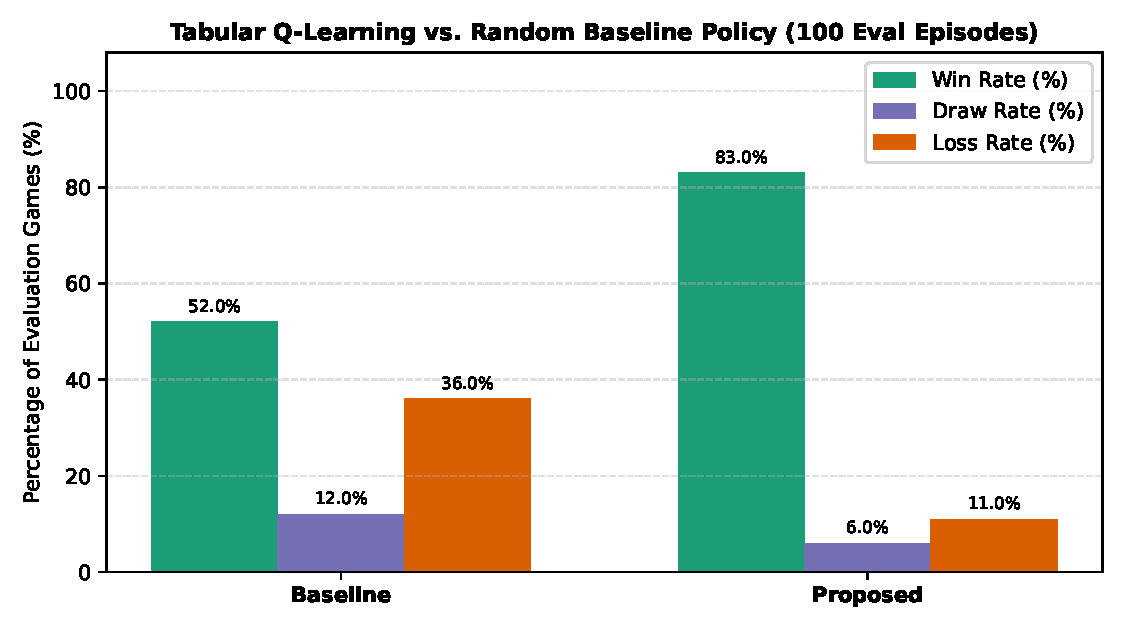
\includegraphics[width=0.86\textwidth]{figures/comparison_chart.pdf}
\caption{Wizualizacja wyników eksperymentalnych wygenerowana przez \texttt{plot\_results.py}.}
\label{fig:comparison_chart}
\end{figure}

\chapter{Rozdział 6: Podsumowanie, Wnioski i Kierunki Rozwoju}
Przeprowadzone eksperymenty w pełni potwierdziły postawioną tezę badawczą. Zaproponowany agent Q-Learning osiągnął współczynnik zwycięstw 0.83 przy odsetku porażek zredukowanym do 0.11, podczas gdy polityka losowa uzyskała jedynie 0.52 wygranych i 0.36 porażek \cite{watkins1992qlearning,sutton2018reinforcement}. Zastosowana czterowarstwowa architektura ADK wyeliminowała halucynacje liczbowe dzięki twardej kompilacji wskaźników symbolicznych.

\bibliographystyle{plain}
\bibliography{references}

\symbolslist{
  $\mathcal{L}$ -- funkcja straty \\
  $\eta$ -- krok uczenia \\
  $\theta$ -- wektor parametrów modelu
}

\abbreviationslist{
  PŁ -- Politechnika Łódzka \\
  ADK -- Artificial-Degree-Printer Development Kit \\
  AST -- Abstract Syntax Tree \\
  SOTA -- State of the Art
}

\definitionslist{
  Neuro-Symbolic Harness -- system łączący generację kodu opartą na modelach językowych z deterministyczną weryfikacją symboliczną.
}

\end{document}
